% 图片模板
\centerline{
    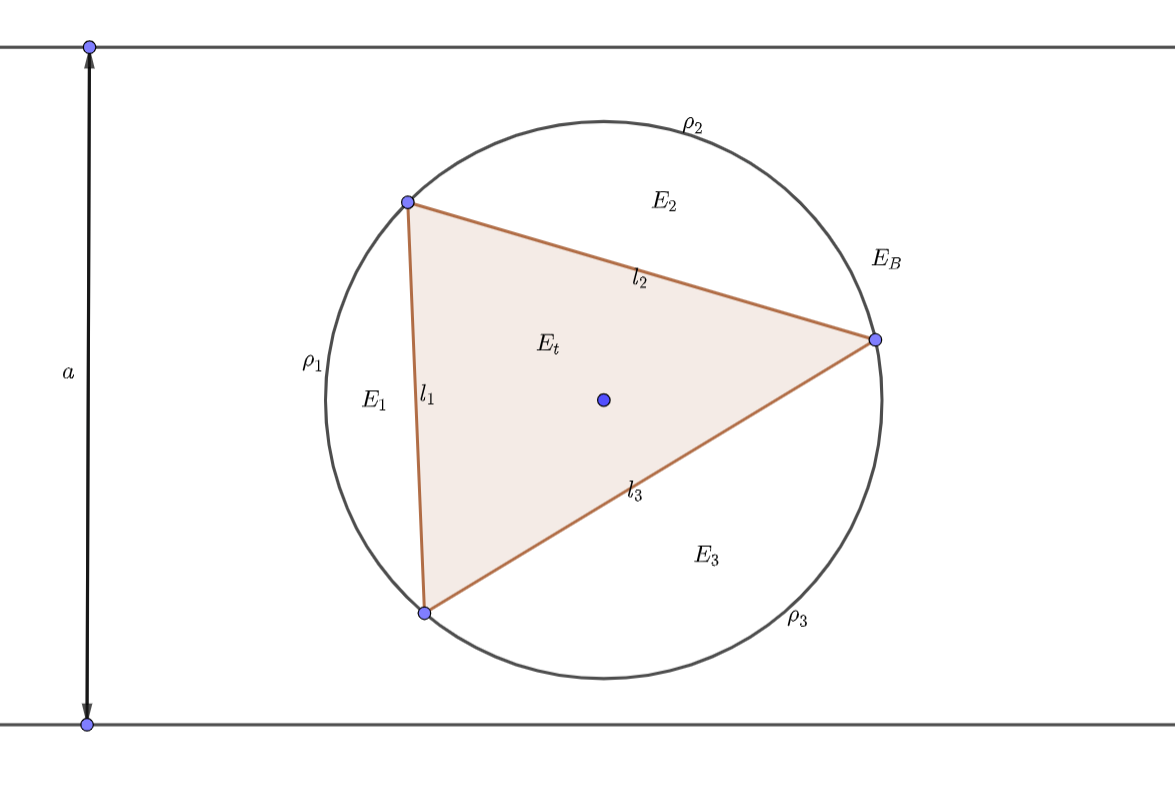
\includegraphics[width=0.8\textwidth]{figure.png}
}
% 表格模板
\renewcommand\arraystretch{0.8} % 设置表格高度为原来的0.8倍
\begin{table}[!htbp] % table标准
    \centering % 表格居中
    \begin{tabular}{p{1cm}<{\centering}p{1cm}<{\centering}p{3cm}<{\centering}p{5cm}<{\centering}} % 设置表格宽度
    %\begin{tabular}{cccc}
        \toprule
        $x_i$ & $f[x_1]$ & $f[x_i,x_{i+1}]$ & $f[x_i,x_{i+1},x_{i+2}]$ \\
        \midrule
        $x_0$ & $f(x_0)$ &                  &                          \\
        $x_0$ & $f(x_0)$ & $f'(x_0)$        &                          \\
        $x_0$ & $f(x_1)$ & $\frac{f(x_1)-f(x_0)}{x_1-x_0}$ & $\frac{f(x_1)-f(x_0)}{(x_1-x_0)^2}-\frac{f'(x_0)}{x_1-x_0}$\\
        \bottomrule
    \end{tabular}
\end{table}

\def\Log{\text{Log}} % 一个简单的宏定义
$\Log$ % 调用方法

%%%% 表格模板 %%%%
\renewcommand\arraystretch{0.8} % 设置表格高度为原来的0.8倍
\begin{table}[!htbp] % table标准
    \centering % 表格居中
    \begin{tabular}{p{1cm}<{\centering}p{1cm}<{\centering}p{3cm}<{\centering}p{5cm}<{\centering}} % 设置表格宽度
    %\begin{tabular}{cccc}
        \toprule
        $x_i$ & $f[x_1]$ & $f[x_i, x_{i+1}]$ & $f[x_i, x_{i+1}, x_{i+2}]$ \\
        \midrule
        $x_0$ & $f(x_0)$ &                  &                          \\
        $x_0$ & $f(x_0)$ & $f'(x_0)$        &                          \\
        $x_0$ & $f(x_1)$ & $\frac{f(x_1)-f(x_0)}{x_1-x_0}$ & $\frac{f(x_1)-f(x_0)}{(x_1-x_0)^2}-\frac{f'(x_0)}{x_1-x_0}$\\
        \bottomrule
    \end{tabular}
\end{table}

%%%% 文字环绕图片, 标题加注释 %%%%
{ % 一般将文字环绕部分的图和文字, 用大括号括起来, 避免对文字外的格式发生影响
\begin{wrapfigure}[13]{r}{.5\linewidth} % 文字环绕行数为13行, 图片靠右 (l为靠左), 图片占0.5的行宽
    \centering
    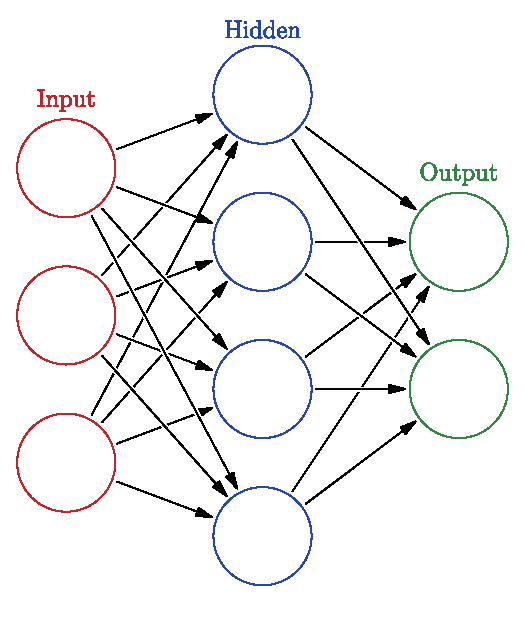
\includegraphics[scale=0.7]{neural_network.eps} % scale=0.7按比例缩放70%
    \caption{神经网络结构\protect\footnotemark[1]} % 记得加\protect, 设置1号脚标
    \label{figure-神经网络结构}
\end{wrapfigure}
\footnotetext[1]{图片来源: \url{https://en.wikipedia.org/wiki/File:Colored_neural_network.svg}}
文字文字
% 这里一定要空一行
}

%%%% 普通图片, 标题加注释 %%%%
\begin{figure}[htbp] % h: 当前位置, t: 顶部, b: 底部, p: 浮动页, 这样组合指的是使用这个顺序进行排版
    \centering
    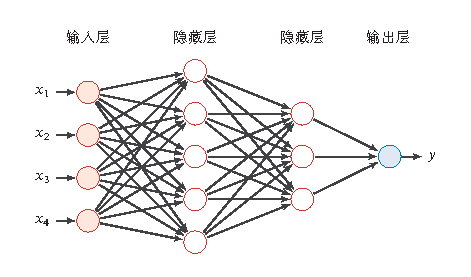
\includegraphics[scale=0.5]{前馈神经网络.eps}
    \caption{前馈神经网络\protect\footnotemark[1]}
    \label{figue-前馈神经网络}
\end{figure}
\footnotetext[1]{图片来源: 邱锡鹏, 神经网络与深度学习 \cite{ref-qxp}, 第92页}

%%%% 两组图并排放(可溢出一些) %%%%
\begin{figure}[htbp]
    \hspace{-2.5cm}
    \subfigure  % 子图的标题
    {
        % 如果一行放三个图改成0.3\linewidth即可
        \begin{minipage}[b]{.62\linewidth}
            \centering
            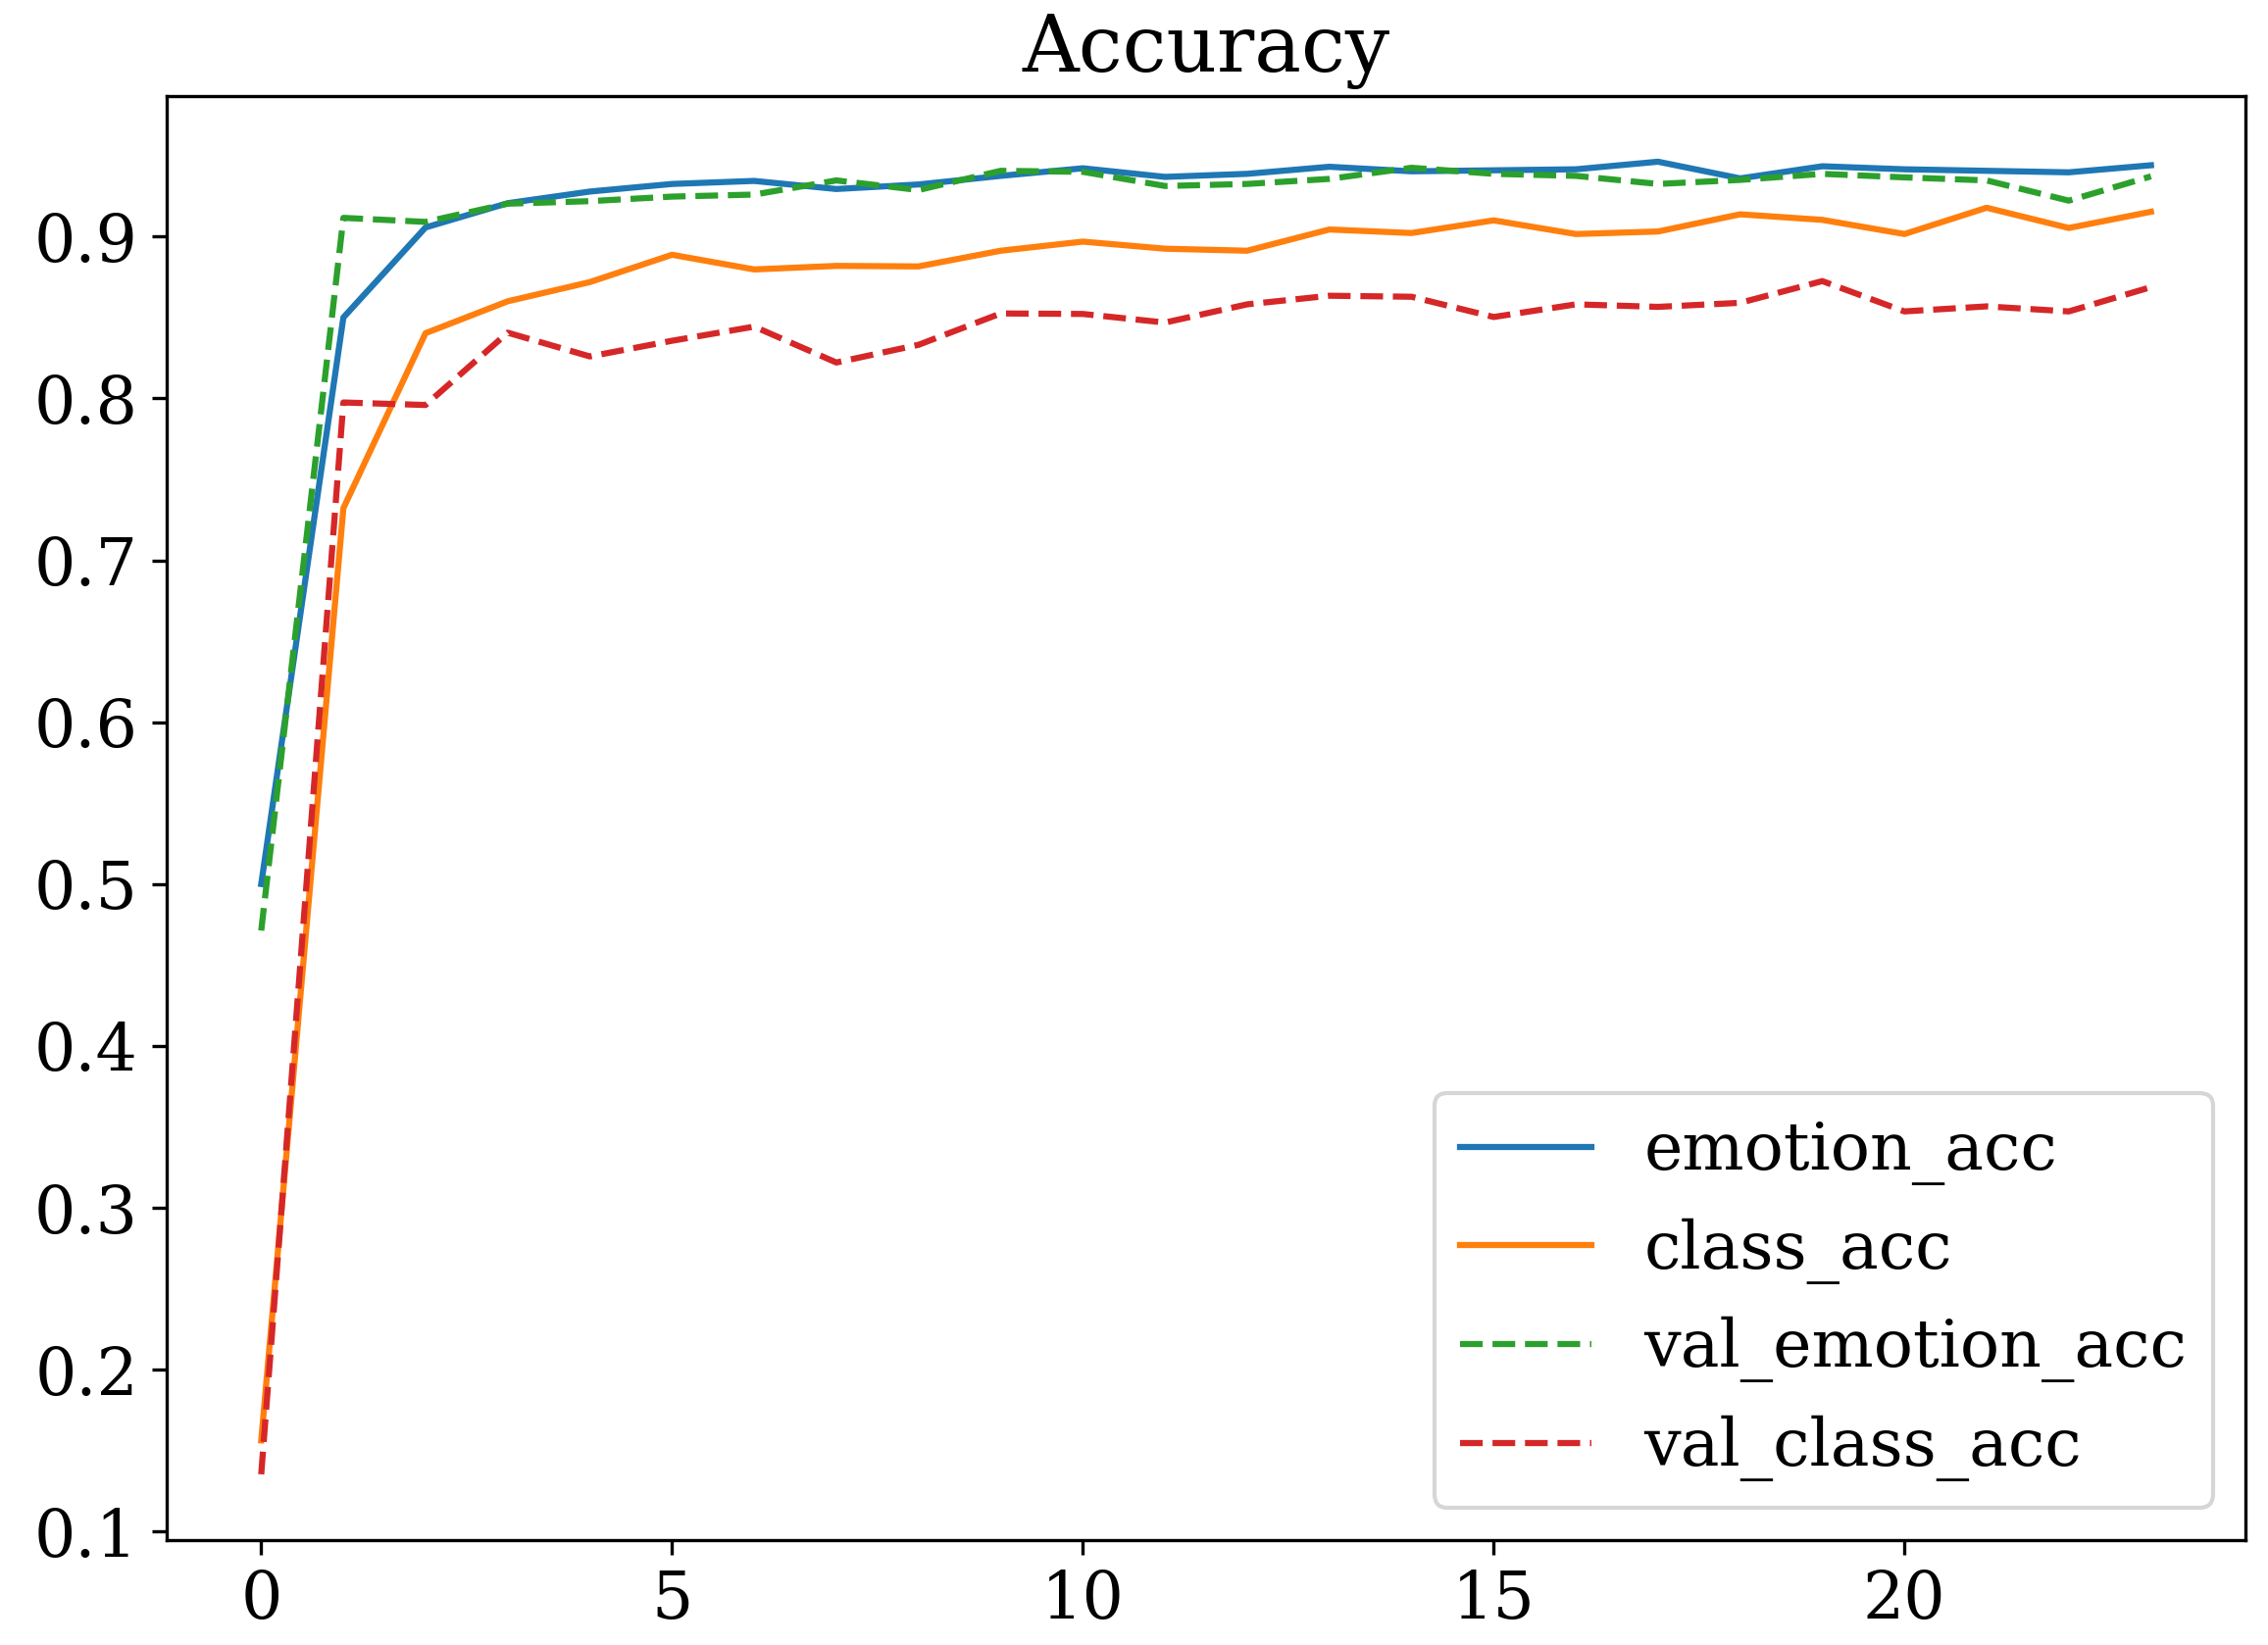
\includegraphics[scale=0.5]{acc_dropout0.1.png}
        \end{minipage}
    }
    \subfigure
    {
        \begin{minipage}[b]{.2\linewidth}
            \centering
            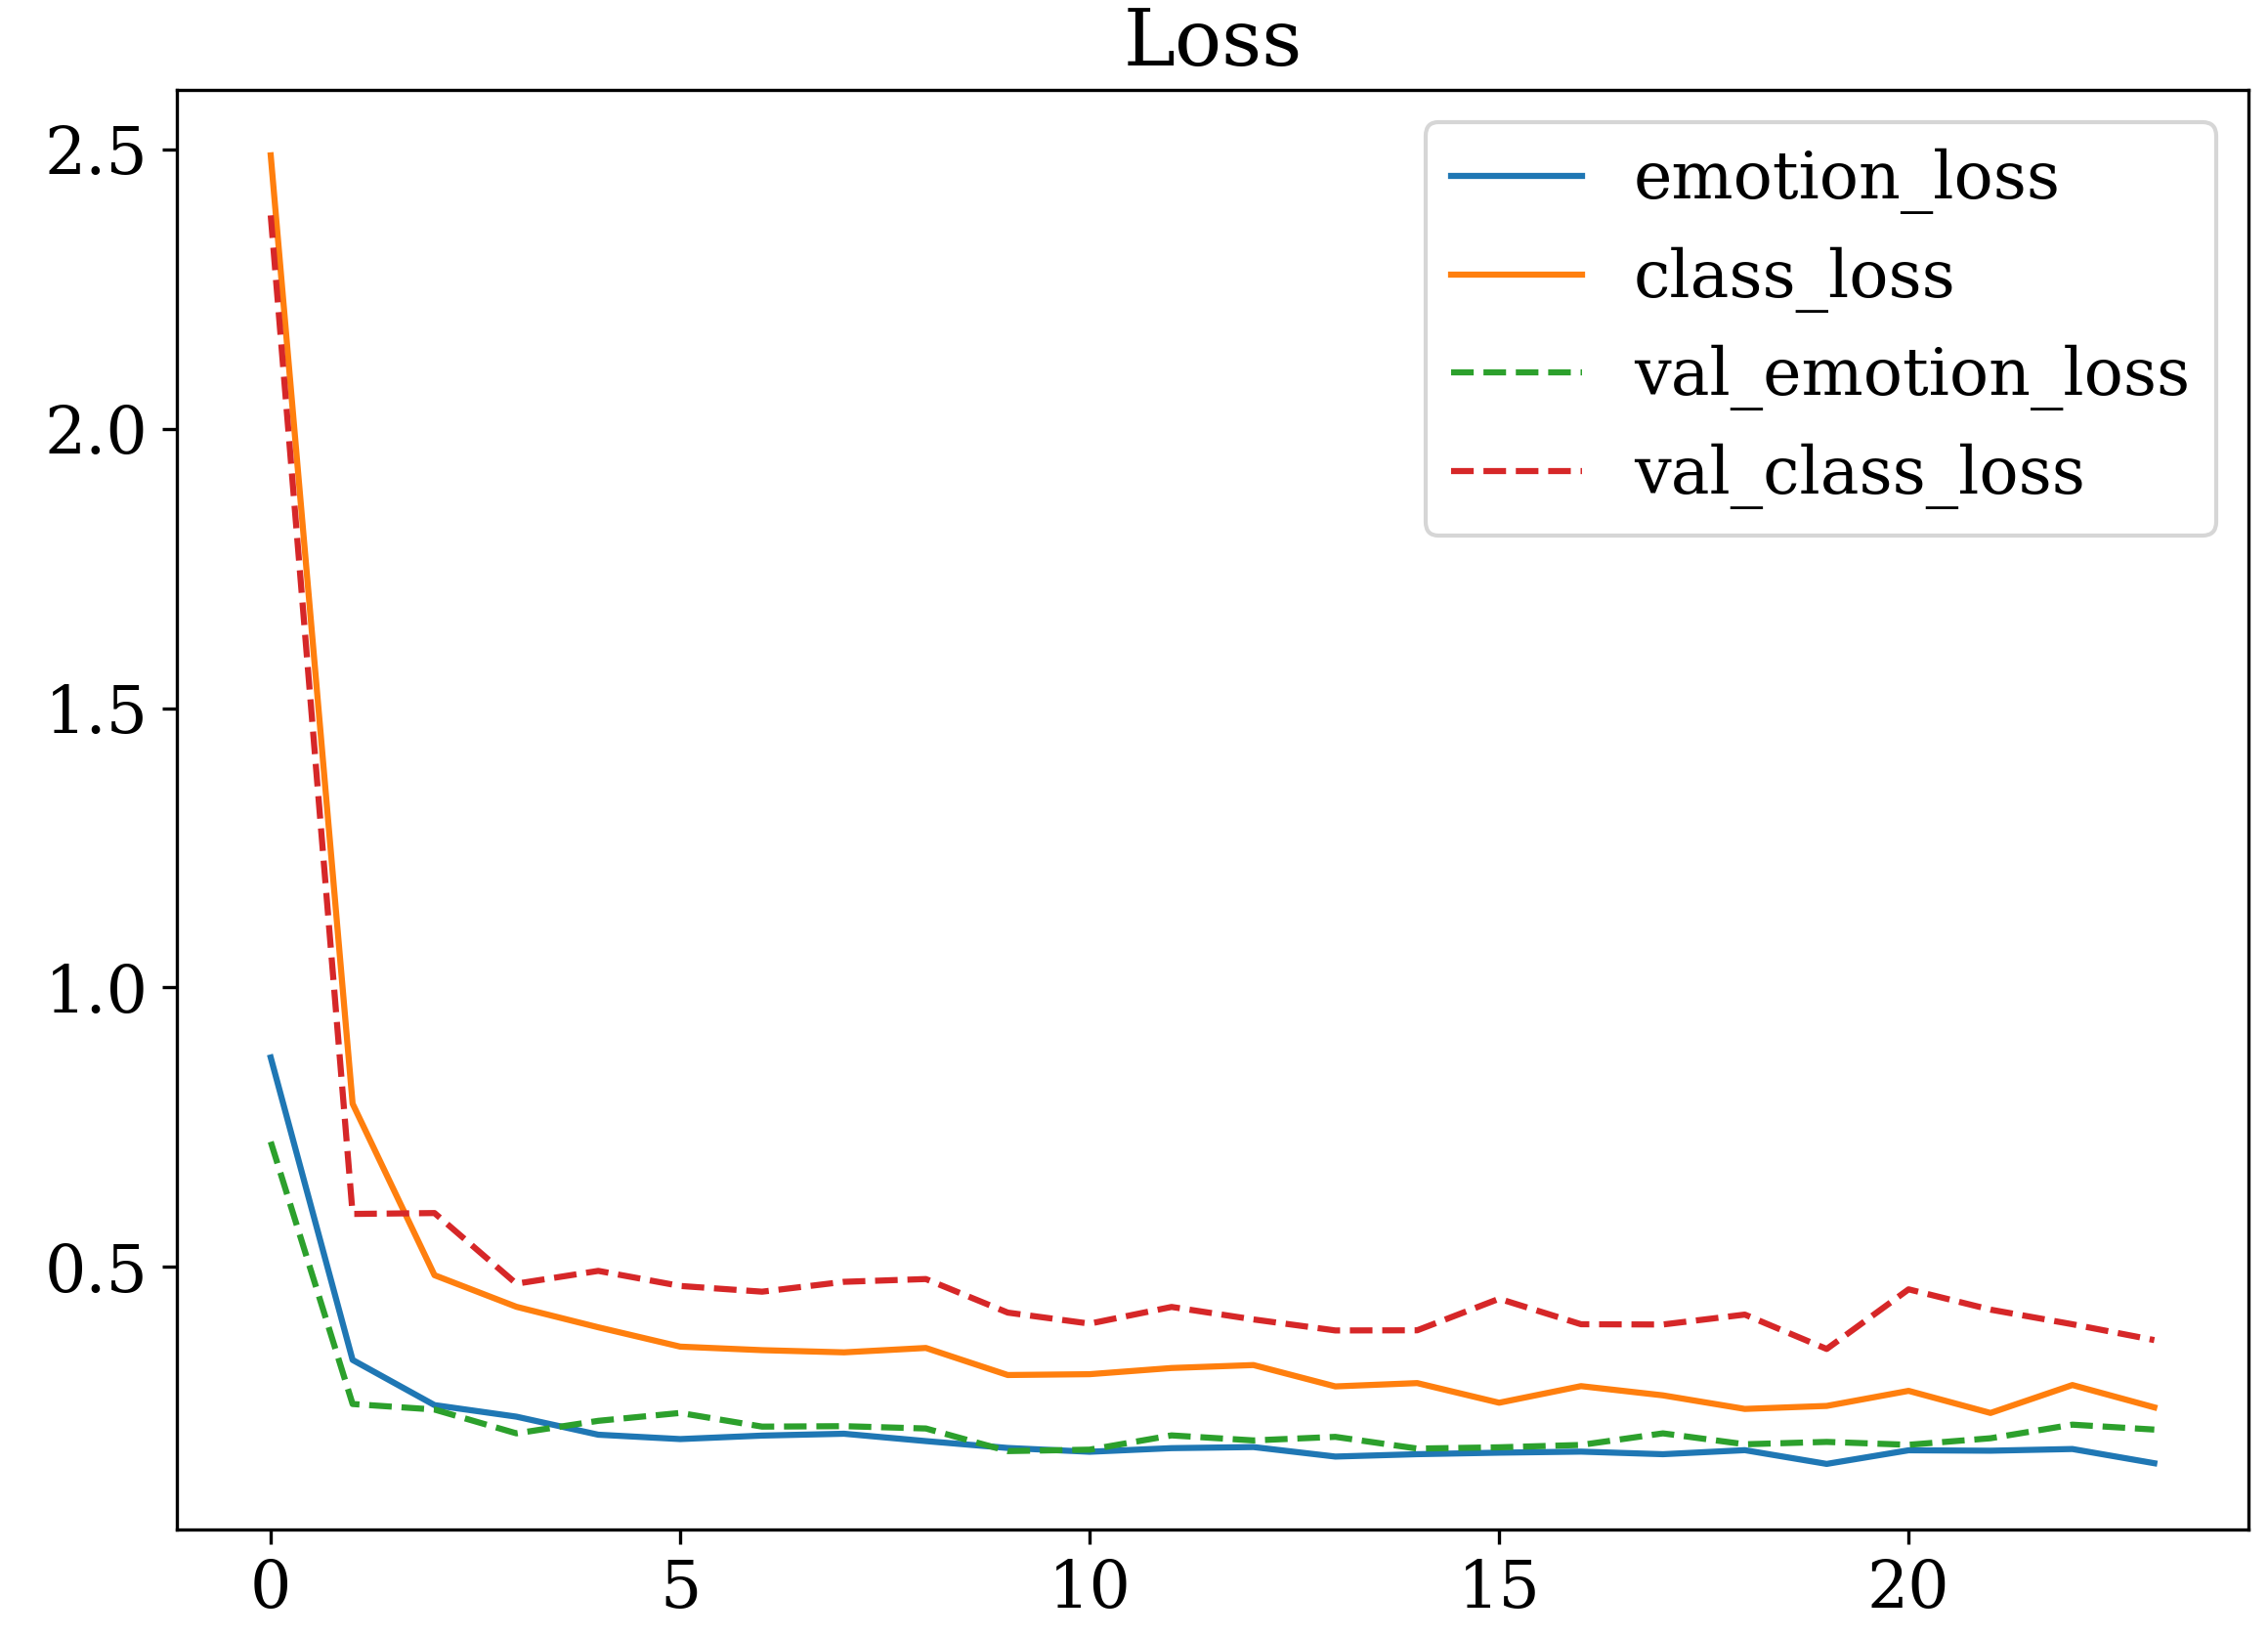
\includegraphics[scale=0.5]{loss_dropout0.1.png}
        \end{minipage}
    }
\end{figure}

%%%% 多组图 %%%%
\begin{figure}[htbp]
    \centering
    \subfigure[迭代1次]  % 子图的标题
    {
        % 如果一行放三个图改成0.3\linewidth即可
        \begin{minipage}[b]{.45\linewidth}  % 0.45排版行距, 即一行放2个图, 一行放不下就换行
            \centering
            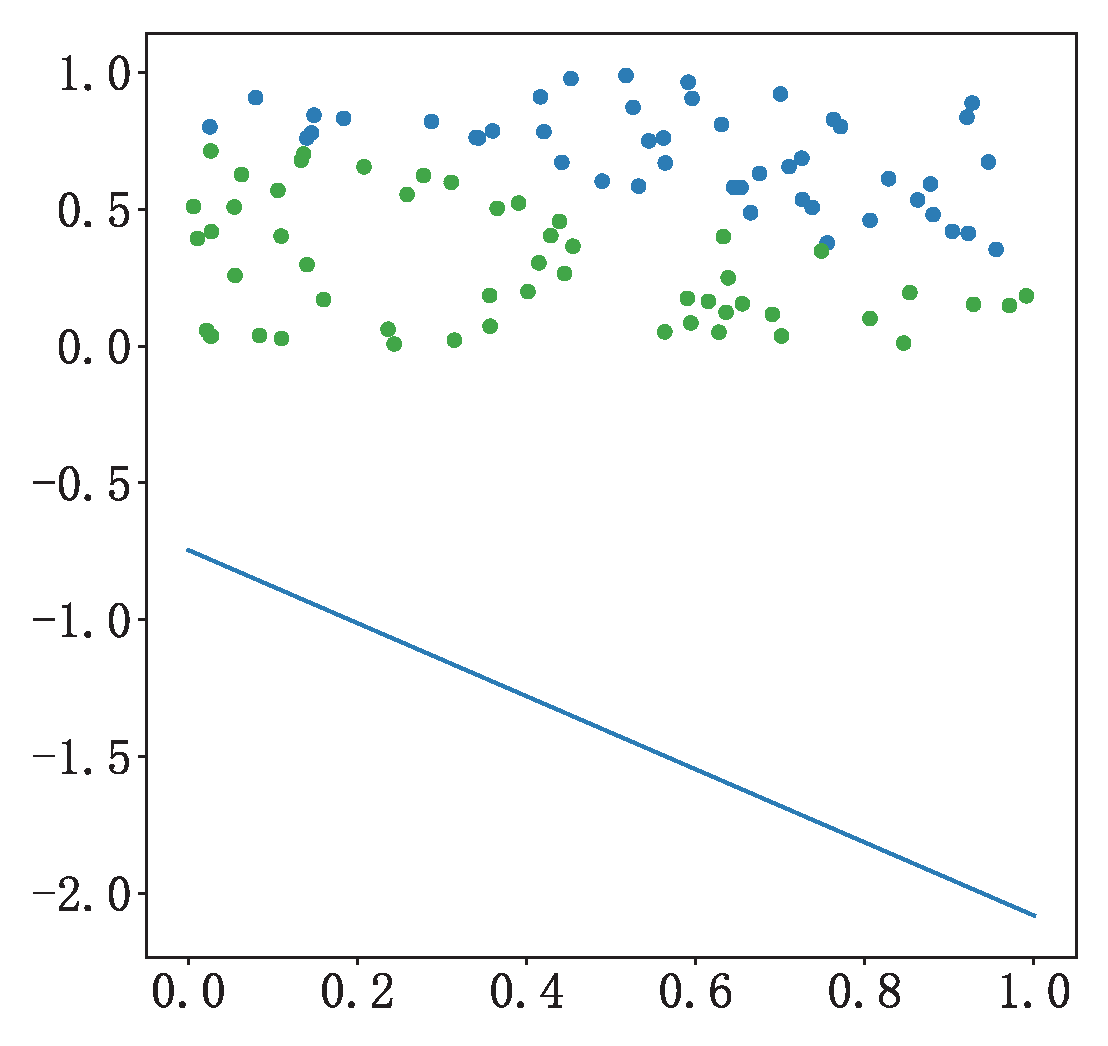
\includegraphics[scale=0.35]{1.eps}
        \end{minipage}
    }
    \subfigure[迭代100次]
    {
        \begin{minipage}[b]{.45\linewidth}
            \centering
            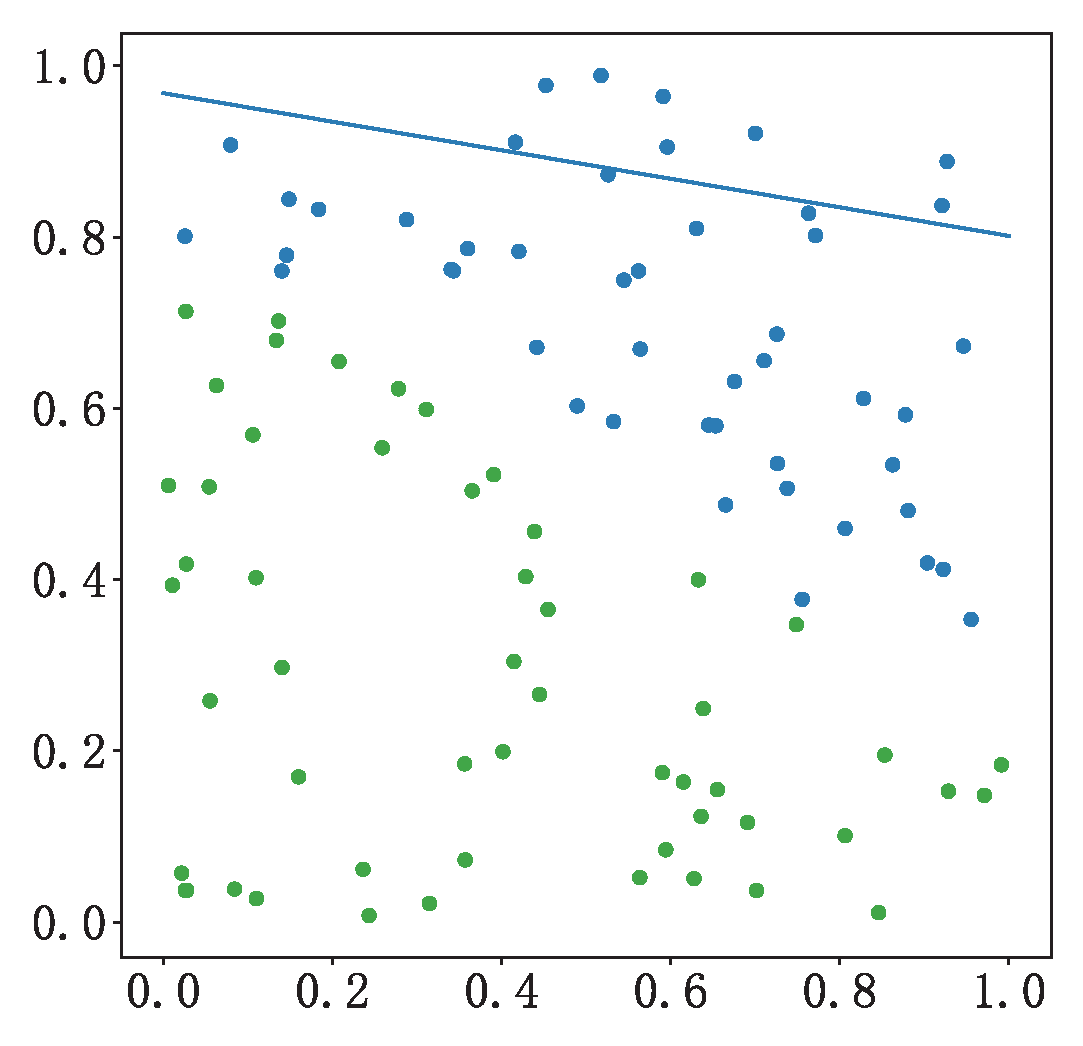
\includegraphics[scale=0.35]{100.eps}
        \end{minipage}
    }
    \subfigure[迭代500次]
    {
        \begin{minipage}[b]{.45\linewidth}
            \centering
            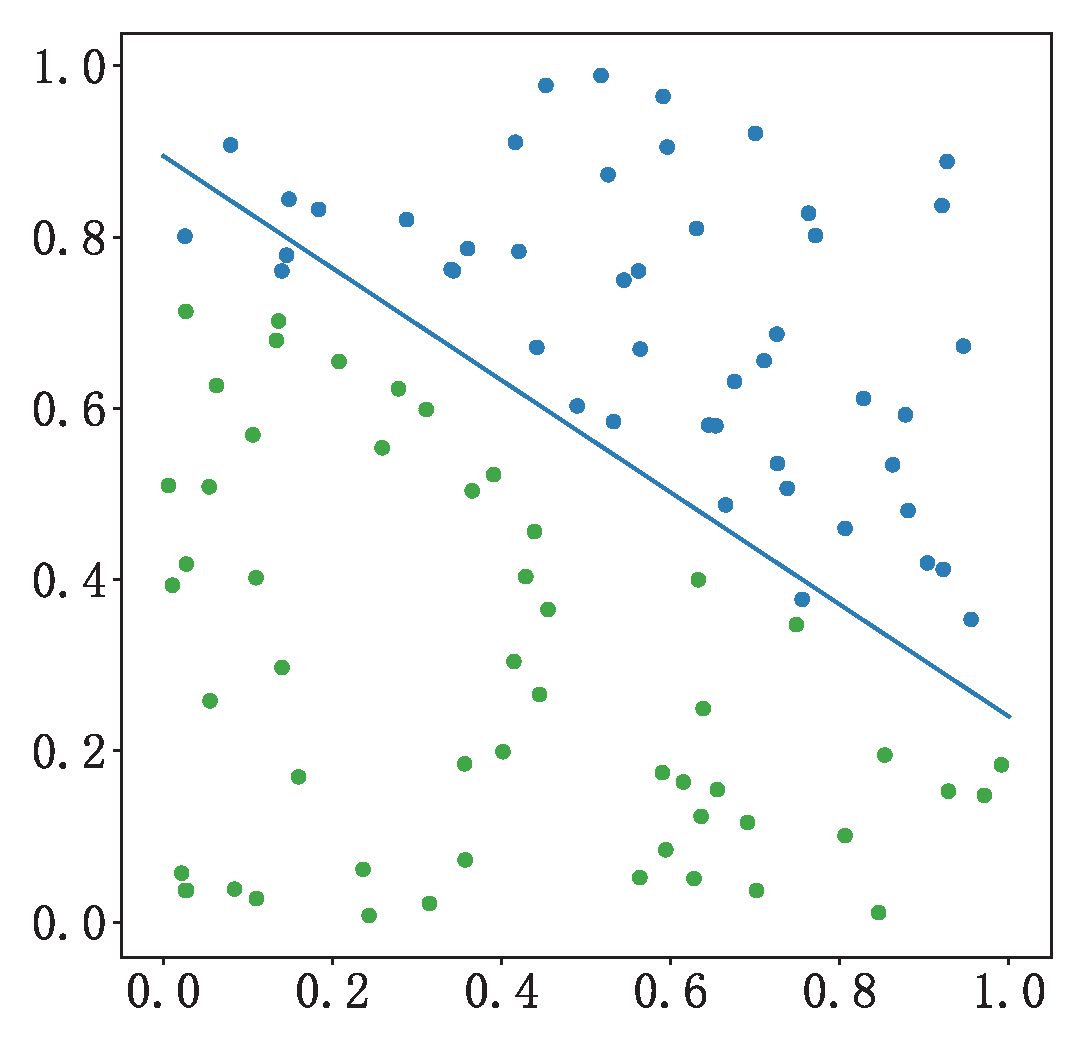
\includegraphics[scale=0.35]{500.eps}
        \end{minipage}
    }
    \subfigure[迭代2000次]
    {
        \begin{minipage}[b]{.45\linewidth}
            \centering
            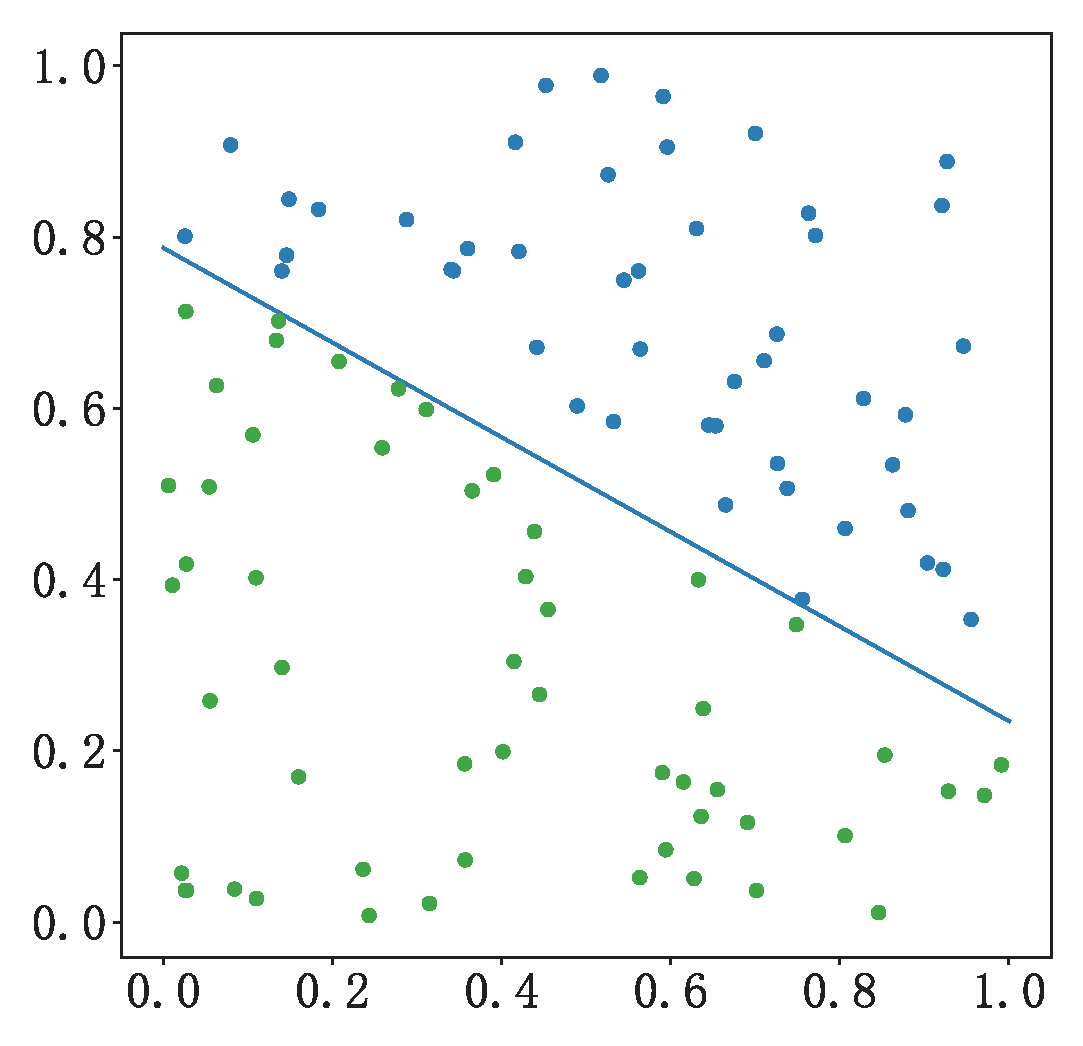
\includegraphics[scale=0.35]{2000.eps}
        \end{minipage}
    }
    \caption{迭代过程图}
    \label{figure-迭代过程图}
\end{figure}